% TODO skratiti arhitekturu

\begin{frame}{CEGIS}
    \begin{itemize}
        \item Program se može sintetisati tako što se definiše specifikacija i zapiše u vidu formule koja se prosledi SMT rešavačima
        \item Koji je najmanji podskup ulaza koji je potrebno razmatrati da bi se sintetisao program koji zadovoljava date specifikacije?
        \item Korišćenjem SMT rešavača dolazimo do svih mogućih implementacija željenog programa koristeći sve ulaze koji su razmatrani do tog trenutka
        \item Paralelno, drugi SMT rešavač pronalazi kontraprimer koji pokazuje da poslednji sintetisani program nije rešenje
    \end{itemize}
\end{frame}

\begin{frame}[fragile]{CEGIS - Arhitektura}
    \begin{itemize}
        \item Pretraga vođena kontraprimerima (eng. \emph{counterexample-guided})
        \item CEGIS se sastoji iz dve faze: \emph{induktivne sinteze} i \emph{verifikacije}
        \item U fazi sinteze se pronalazi program kandidat koji može da zadovolji specifikaciju
        \item U fazi verifikacije se proverava da li taj kandidat zaista zadovoljava specifikaciju
    \end{itemize}
    \begin{figure}
        \begin{center}
            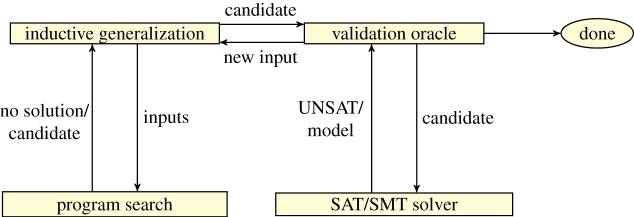
\includegraphics[scale=0.4]{../resources/cegis.jpeg}
        \end{center}
        \caption{CEGIS petlja}
    \end{figure}
\end{frame}

\begin{frame}{CEGIS}
    \begin{itemize}
        \item Da bismo u potpunosti definisali CEGIS sintezu programa, potrebno je odgovoriti na sledeća pitanja:
        \begin{itemize}
            \item Kako treba da izgleda specifikacija traženog programa?
            \item Kako ćemo vršiti sintezu programa kandidata?
            \item Kako da proverimo da li program kandidat zadovoljava specifikacije?
            \item Kako da prosledimo povratne informacije za buduće kandidate?
        \end{itemize}
    \end{itemize}
\end{frame}
